% !Mode:: "TeX:UTF-8"
% VL 1, gebaut aus part-grundlagen/01-was-ist-deep-learning.md
% (Wochenzuordnung: kurs-2026-27.md; Zeitverteilung und Dialogmuster:
%  transcripts/vl01-ueberblick-2025/notiz.md).
%
% Wenig Text auf den Folien, die Ausführung steht in \note{} — die Folie ist der
% Gesprächsanlass, nicht das Handout.
% !Mode:: "TeX:UTF-8"
\newcommand{\thepage}{} % to silence a hyperref warning about pdfpagelabels
\RequirePackage[]{silence}
\WarningsOff[hyperref]
\PassOptionsToPackage{log-declarations=false}{xparse}
%\RequirePackage[l2tabu, orthodox]{nag}
\RequirePackage{luatex85} % to make \pdf...= commands work with LuaTeX
\documentclass[aspectratio=169,t]{beamer}
\usepackage{ifthen}
\usepackage[T1]{fontenc}
\usepackage{iftex}
\ifLuaTeX
 \usepackage{fontspec}
 \setmainfont[Ligatures=TeX]{Source Sans Pro}
\else
 \usepackage[utf8]{inputenc}
\fi
\usepackage{german}
\usepackage{newunicodechar}
\newunicodechar{€}{\texteuro}
\newunicodechar{ß}{\ss}
\renewcommand{\SS}{\iffontchar\font"1E9E \symbol{"1E9E}\else SS\fi}
\usepackage{ellipsis}
\usepackage{microtype}
\usepackage{listings}
\usepackage{sourcecodepro}
\lstset{language=Python, basicstyle=\ttfamily}
\usepackage{amsfonts}
\usepackage{amssymb}
\usepackage{amsthm}
\usepackage{fancyhdr}
\usepackage{graphicx}

\newtheorem{proposition}[theorem]{Proposition}

\DeclareMathOperator*{\argmax}{argmax}
\DeclareMathOperator{\supp}{supp}
\newcommand{\E}{\ensuremath{\mathbb{E}}}
\newcommand{\V}{\ensuremath{\mathbb{V}}}

\setbeamercolor{emph}{fg=purple}
\renewcommand<>{\emph}[1]{%
  {\usebeamercolor[fg]{emph}\only#2{\itshape}#1}%
}



\hypersetup{draft=false,colorlinks=false,pdfpagemode=UseOutlines,plainpages=false,
            breaklinks=true,bookmarksnumbered=true,pdfborder=0 0 0,
            pdftitle={Einführung in Deep Learning WiSe 2026/27 HHU},
            pdfauthor={Konrad Voelkel},
            pdfsubject={data science}}

%\documentclass[aspectratio=169,t]{beamer}
\usetheme{hhubeamer} % put the hhu-beamer-theme in /usr/share/texmf/tex/latex/beamer/themes/

% -------------------- Code listings config --------------------
% Define custom colors for syntax highlighting
\definecolor{codegreen}{rgb}{0,0.6,0}
\definecolor{codegray}{rgb}{0.5,0.5,0.5}
\definecolor{codepurple}{rgb}{0.58,0,0.82}
\definecolor{backcolour}{rgb}{0.96,0.96,0.94} % Very light gray/beige
% Configure the listings package
\lstset{
    language=Python,
    backgroundcolor=\color{backcolour},   
    commentstyle=\color{codegreen}\itshape,
    keywordstyle=\color{blue}\bfseries,
    numberstyle=\tiny\color{codegray},
    stringstyle=\color{codepurple},
    basicstyle=\ttfamily\footnotesize, % Use a monospaced font
    breakatwhitespace=false,         
    breaklines=true,      
             % Enable automatic line breaking
    captionpos=b,                      % Caption at the bottom
    keepspaces=true,                 
    numbers=left,                      % Line numbers on the left
    numbersep=10pt,                    % Distance of line numbers from the code
    showspaces=false,                
    showstringspaces=false,            % Don't show weird underscores in strings
    showtabs=false,                  
    tabsize=4,
    frame=single,                      % Add a subtle border around the code
    rulecolor=\color{black!20},        % Border color
  }

\event[]{}
\author[Wintersemester 2026/27]{Dr. Konrad Völkel, Wintersemester 2026/27}

%\title{Data Science, VL 1}
%\date{16.04.2026}


%%% Local Variables:
%%% mode: latex
%%% TeX-master: t
%%% End:


% Fassung mit Dozentennotizen (zweiter Schirm): die nächste Zeile einkommentieren.
% Muss nach dem Header stehen, der lädt die Dokumentklasse.
% \setbeameroption{show notes on second screen=right}

\graphicspath{{../images/}}

\title[Was ist Deep Learning? (VL 1)]{Was ist Deep Learning?\\\large Einführung in Deep Learning, VL 1}
\date{14.10.2026}

\begin{document}

\begin{frame}
  \titlepage

  \note{\textbf{Ablauf, 90 Minuten.} Die Zahlen sind \emph{Seiten} wie in der Fußzeile,
    nicht Rahmen: Mehrere Folien bauen sich schrittweise auf (im Quelltext
    \texttt{\% Transition}).\\[2pt]
    \begin{tabular}{@{}rll@{}}
      0--5   & Seiten 1--3   & Organisatorisches, Material\\
      5--12  & Seiten 4--6   & Voraussetzungen, Lernziele (Handzeichen)\\
      12--23 & Seite 6       & \textbf{Umfrage live in ILIAS}\\
      23--26 & Seiten 7--8   & Definition\\
      26--37 & Seite 9       & Semesterplan -- der lange Block, lebt von Rückfragen\\
      37--43 & Seiten 10--11 & Python: Provokation und Auflösung\\
      43--51 & Seiten 12--15 & Daten, erzeugende Verteilung, GMM\\
      51--57 & Seiten 16--19 & Supervised, Regression, Klassifikation\\
      57--62 & Seiten 20--21 & Modellgüte: Split, die vier Maße\\
      62--68 & Seiten 22--25 & \textbf{Zwei Prüfungsfragen} (Peer Instruction, je 3 Min.)\\
      68--76 & Seiten 26--27 & \textbf{Quizfrage} (Dialog), Auflösung\\
      76--81 & Seiten 28--31 & \textbf{Lesetext}: Zitat, eine Frage, Leseauftrag\\
      81--86 & Seiten 32--35 & Kurzgeschichte\\
      86--88 & Seiten 36--39 & Take-Home, Themenfelder A/B/C\\
      88--90 & Seiten 40--41 & In die Praxis, Danke und Fragen
    \end{tabular}\\[4pt]
    \textbf{Enger als 2025}: Definitionsfolie und zwei Prüfungsfragen kosten rund fünf
    Minuten. Bezahlt aus je einer Minute bei Semesterplan, Python und Supervised und aus
    der \emph{Kurzgeschichte} (8 auf 5 Min.); der Lesetext ist dafür \emph{billiger}
    als 2025 (fünf statt acht Minuten, ohne Browser).
    \textbf{Gerechnet, nicht gemessen} -- an der Aufzeichnung nachjustieren.\\[2pt]
    \textbf{Wenn die Zeit knapp wird}, in dieser Reihenfolge kürzen: den Leseauftrag
    (27) nur ansagen statt vorzulesen; die zweite Prüfungsfrage (20--21) überspringen,
    sie wiederholt die erste rechnerisch; Python auf eine Seite zusammenziehen;
    Kurzgeschichte ab 2015 überspringen.
    \textbf{Wenn Zeit übrig ist}: Quizfrage, Semesterplan und die beiden Prüfungsfragen
    vertragen beliebig viel Dialog.}
\end{frame}

% ------------------------------------------------------------------ Formalia
\begin{frame}
  \frametitle{Organisatorisches}

  \begin{itemize}\setlength{\itemsep}{6pt}
  \item Übung: \emph{15.10.2026} um 10:30 (morgen), 25.22.U1.52
  \item Blätter wöchentlich, Abgabe Mi 12:00
  \item Zulassung: 8 bestandene Blätter
  \item Klausur: 11.02.2027
  \item Note: nur die Klausur, ohne Hilfsmittel
  \item Fragen in den Chat: \texttt{\#eidl-2026}
  \end{itemize}

  \note{Vier Minuten, nicht mehr -- die Details stehen auf der ILIAS-Kursseite.
    Betonen: die Übung fängt schon morgen an. Fragen gehören in den Rocket.Chat-Kanal
    \texttt{\#eidl-2026}, inhaltliche wie organisatorische -- nicht in mein Postfach,
    dann haben alle etwas davon. Der Einladungslink steht auf der ILIAS-Kursseite;
    hier kurz zeigen, wie man beitritt. „Bestanden“ heißt mindestens die Hälfte der
    Punkte; statt eines letzten Blatts gibt es eine Probeklausur. Zweitklausur ist
    am 15.03.2027. Die Blätter sind Studienleistung und werden von Elisa Kleinfeld
    korrigiert; die Note kommt allein aus der Klausur.}
\end{frame}

\begin{frame}
  \frametitle{Material}

  \begin{itemize}\setlength{\itemsep}{6pt}
  \item \emph{Neu}: Skript zur Vorlesung\\
    {\small\url{voelkel.pages.cs.uni-duesseldorf.de/eidl-skript/}}
  \item Folien vorab in ILIAS
  \item Lösungshinweise nach Abgabeschluss
  \item Aufzeichnungen aus 2025/26 in der Mediathek
  \item \emph{Neu}: Aufzeichnungen aus 2026/27 -- mit diesem Foliensatz
  \end{itemize}

  \note{Das Skript ist die Neuerung gegenüber den Vorjahren: es deckt den Stoff ab und
    geht an einigen Stellen darüber hinaus, mit Vertiefungsboxen zum Aufklappen.
    Wer die Vorlesung verpasst, liest das Kapitel. Ausdrücklich um Fehlermeldungen bitten.
    Tafelanschriebe gibt es nicht digital. Zum Weiterlesen frei verfügbar: Prince,
    \emph{Understanding Deep Learning}, und Deisenroth/Faisal/Ong, \emph{MML} --
    beide sind im Skript pro Kapitel verlinkt.}
\end{frame}

% ------------------------------------------------------------------ Voraussetzungen
\begin{frame}
  \frametitle{Keine Angst vor:}

  \begin{center}
    \Large
    Vektor \quad Matrix \quad Ableitung\\[8pt]
    Zufallsvariable \quad lineare Regression\\[8pt]
    Python mit NumPy
  \end{center}

  \note{Handzeichen einsammeln: Wer hat Data Science gehört? Wer hat schon mal ein
    neuronales Netz trainiert? Das gibt mir ein Bild vom Raum und ihnen das Gefühl,
    nicht allein zu sein.
    „Keine Angst vor“ heißt nicht „auswendig können“. Wer bei der Ableitung zuckt,
    bekommt in VL 5/6 ein Problem -- lieber jetzt auffrischen.
    Machine Learning und Data Science 2 sind \emph{nicht} nötig.}
\end{frame}

\begin{frame}
  \frametitle{Was wir zusammen lernen}

  \begin{itemize}\setlength{\itemsep}{6pt}
  \item Wie ein neuronales Netz arbeitet
  \item Wie ein neuronales Netz lernt
  \item PyTorch
  \item Fertige Modelle benutzen -- und verändern
  \item Text und Bilder
  \item Wie man Katzen von Hunden unterscheidet
  \end{itemize}

  \note{Die Begriffe dahinter: Gradientenabstieg, Loss-Funktion, Matrizen- und
    Tensorkalkül, latenter Raum, logistische Regression -- die kann man hier
    aufzählen, sie stehen bewusst nicht auf der Folie.
    2025 kamen aus der Umfrage (mit ChatGPT geclustert) genau diese vier Wünsche
    zurück. Das kann man sagen, es nimmt der Liste das Beliebige.}
\end{frame}

% ------------------------------------------------------------------ Umfrage
\begin{frame}
  \frametitle{Eingangsumfrage}

  \begin{center}
    \Huge Was ist für Sie\\[6pt] Deep Learning?
  \end{center}

  \note{\textbf{Browser-Block, etwa zehn Minuten, live in ILIAS} -- wie 2025.
    Die Umfrage läuft seit Anfang Oktober, hier die Ergebnisse gemeinsam durchgehen:
    Vorkenntnisse, die eigenen Definitionen, Interessen, Anwesenheitsabsicht.
    Die \emph{falschen} Definitionen sind der Einstieg: gemeinsam korrigieren,
    nicht von mir vortragen. Daraus fällt die Definition auf der nächsten Folie
    fast von selbst heraus.
    Wer die Umfrage noch nicht ausgefüllt hat: jetzt, dauert zwei Minuten.}
\end{frame}

% ------------------------------------------------------------------ Definition
\begin{frame}
  \frametitle{Der Name ist erfreulich ehrlich}

  \begin{columns}[c]
    \begin{column}{0.52\textwidth}
      \Large
      \emph{deep} = viele Ebenen (Layer)\\[10pt]
      \emph{learning} = Training\\[18pt]
      \pause % Transition 2026-10-14: erst fragen lassen, dann zusammensetzen
      \normalsize Training künstlicher neuronaler Netze\\mit vielen Ebenen.
    \end{column}
    \begin{column}{0.44\textwidth}
      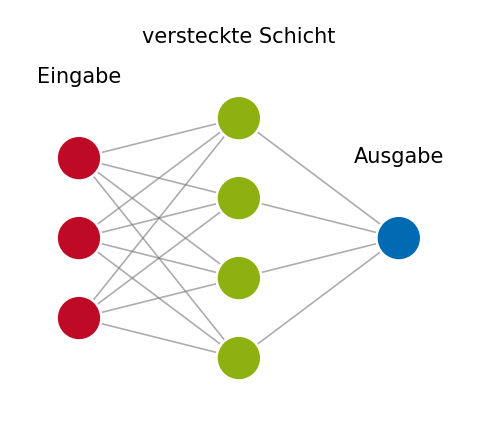
\includegraphics[width=\textwidth]{vl01-mlp.png}
    \end{column}
  \end{columns}

  \note{Take-Home-Message der Sitzung: Deep Learning ist der Teil von Machine Learning,
    der tiefe neuronale Netze einsetzt -- nicht mehr und nicht weniger. Kein Bewusstsein,
    keine Magie, keine Definition von „KI“ nötig.
    Rückfrage in den Raum: Was ist dann eine Ebene? Was heißt Training? -- genau das
    ist der Inhalt des Semesters, und hier beginnt der Semesterplan.}
\end{frame}

% ------------------------------------------------------------------ Semesterplan
\begin{frame}
  \frametitle{Der grobe Plan}

  \begin{columns}[t]
    \begin{column}{0.5\textwidth}
      \begin{enumerate}\setlength{\itemsep}{1pt}
      \item Was ist Deep Learning? (heute)
      \item Neuron und Perzeptron
      \item Vortrainierte Modelle, Tensoren
      \item Logistische Regression
      \item Loss und Gradientenabstieg
      \item Backpropagation
      \item Netze von Hand bauen
      \item Autoencoder
      \end{enumerate}
    \end{column}
    \begin{column}{0.5\textwidth}
      \begin{enumerate}\setlength{\itemsep}{1pt}\setcounter{enumi}{8}
      \item VAE, word2vec, Graphen
      \item RNNs und Transformer
      \item Faltung und CNNs
      \item Autograd, LLMs benutzen
      \item GANs
      \item Latente Räume, Anwendungen
      \item Destillation, Vibecoding
      \end{enumerate}
    \end{column}
  \end{columns}

  \note{Zwölf Minuten -- der längste Block der Sitzung, weil 2025 zu jedem Stichwort
    eine Frage kam. Das ist gut so: hier entsteht die Landkarte, an die der Rest
    angehängt wird. Aufhänger: Mark-I-Perzeptron (echte Hardware!), Hugging Face,
    „was ist ein latenter Raum“.
    Nicht dabei und ausdrücklich sagen: Transformer selbst trainieren, große echte
    Daten, Optimierungstheorie, CUDA-Programmierung, Reinforcement Learning.}
\end{frame}

% ------------------------------------------------------------------ Python
\begin{frame}
  \frametitle{Python ist eine Katastrophe}

  \begin{center}
    \Large
    single-threaded, GIL\\[6pt]
    interpretiert\\[6pt]
    dynamisch typisiert\\[6pt]
    nicht maschinennah
  \end{center}

  \note{Als Provokation stehen lassen und \emph{nicht} sofort auflösen.
    Frage in den Raum: Wenn das alles stimmt -- warum ist dann jedes ML-Framework
    in Python? Antworten sammeln, dann umblättern.
    Details, falls sie kommen: Garbage Collection und GIL erschweren Multithreading;
    Typechecking zur Laufzeit; SIMD-Register und Cachegrößen sind aus Python heraus
    schwer zu nutzen.}
\end{frame}

\begin{frame}
  \frametitle{Python ist perfekt}

  \begin{center}
    \Large
    Rapid Prototyping\\[6pt]
    Rechnen in C, Rust, CUDA\\[6pt]
    riesiges Ökosystem\\[6pt]
    Gewichte sind sprachunabhängig
  \end{center}

  \bigskip
  \begin{center}
    Python ist die \emph{Steuersprache}.
  \end{center}

  \note{Die Auflösung ist der Punkt, nicht die Listen: die Arbeit --
    Matrixmultiplikationen auf Millionen von Zahlen -- passiert in kompiliertem
    Code, oft auf der GPU. Python sagt nur, welche Operation als Nächstes dran ist.
    Genau das ist die Idee der vektorisierten Programmierung mit NumPy; PyTorch
    treibt sie weiter. Beide Python-Folien zusammen: sechs Minuten.}
\end{frame}

% ------------------------------------------------------------------ ML-Begriffe
\begin{frame}
  \frametitle{Erinnerung: Woher kommen die Daten?}

  \begin{center}
    \Large
    $x_1, \dots, x_N \in \mathbb{R}^n$\\[14pt]
    \normalsize gezogen aus einer \emph{erzeugenden Verteilung} $X$,\\
    die wir nicht kennen.
  \end{center}

  \pause % Transition 2026-10-14
  \bigskip
  \begin{center}
    Ein \textbf{Modell} beschreibt sie: als Dichte $p(x)$ -- oder als \emph{Sampler}.
  \end{center}

  \pause % Transition 2026-10-14: die Warnung zuletzt, sie widerspricht dem eben Gesagten
  \bigskip
  \begin{center}
    \small
    \emph{Achtung}: „Modell“ ist auch ein gängiger Name für konkrete neuronale Netze.
  \end{center}

  \note{\textbf{Die Warnung am Ende ernst nehmen, sie ist der häufigste stille
    Stolperstein des Semesters.} „Modell“ heißt hier die Beschreibung einer Verteilung --
    und zwei Folien später heißt „Modell“ das trainierte Netz, also einfach ein Satz
    Gewichte. Beides ist üblich, beides bleibt, und niemand sagt dazu, welches gemeint
    ist. Wer im Zweifel ist, fragt: Beschreibt das Ding eine Verteilung, oder rechnet es
    eine Vorhersage aus?
    Die Komponenten von $x_i$ heißen Features; die Grundannahme des maschinellen
    Lernens ist, dass die Daten eine Stichprobe aus einer Population sind.
    Ein Modell mit Sampler heißt \textbf{generativ}.
    Frage in den Raum, die 2025 gut lief: Ich habe eine Dichte -- wie komme ich
    damit zu Stichproben? Antwort: Rejection Sampling, Monte-Carlo. Steht bewusst
    nicht im Skript, ist aber die Brücke zwischen den beiden Beschreibungen.}
\end{frame}

\begin{frame}
  \frametitle{Ein generatives Modell in Aktion}

  \begin{center}
    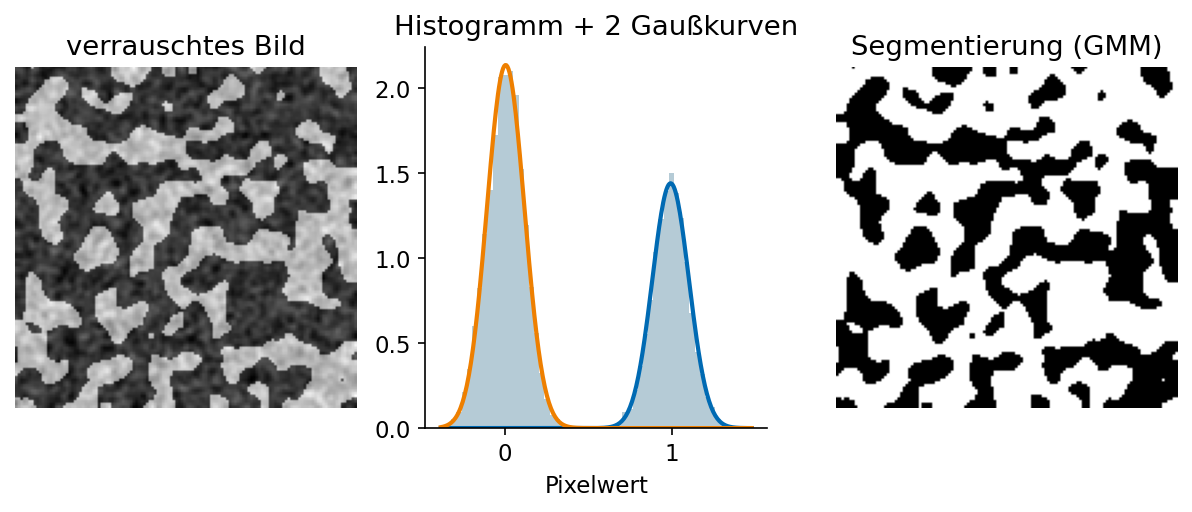
\includegraphics[width=0.8\textwidth]{vl01-gmm-segmentation.png}
  \end{center}

  \note{Kein Deep Learning, ganz bewusst: ein generatives Modell kann sehr klein sein.
    Ein Gaussian Mixture Model mit zwei Komponenten wird an das Histogramm der
    Pixelwerte gefittet -- zwei Gauß-Kurven, ein Schnittpunkt, fertig ist die
    Segmentierung in Vorder- und Hintergrund.
    Frage: Was wäre hier das „Training“, was die „Inferenz“?}
\end{frame}

\begin{frame}
  \frametitle{Supervised und Unsupervised}

  \begin{center}
    \Large
    mit Labels $y_i$ \quad$\longrightarrow$\quad supervised\\[10pt]
    ohne Labels \quad$\longrightarrow$\quad unsupervised
  \end{center}

  \pause % Transition 2026-10-14
  \bigskip
  \begin{center}
    \normalsize
    \textbf{Training}: Daten $\to$ Gewichte \qquad
    \textbf{Inferenz}: neue Daten + Gewichte $\to$ Vorhersage
  \end{center}

  \note{Take-Home: Supervised heißt, ich habe in den Trainingsdaten eine Spalte,
    die ich später nicht mehr bekomme und vorhersagen will.
    Unsupervised: generative Modelle wie eben, Clustering, Dimensionsreduktion.
    Oft ist $y_i \in \mathbb{R}$ (Regression) oder $y_i \in \{0,1\}$ (binäre Klassifikation).
    „Gefittetes Modell“ heißt bei uns immer: ein Satz Zahlen.}
\end{frame}

\begin{frame}
  \frametitle{Regression und Klassifikation}

  \begin{center}
    \Large
    $Y = f(X) + \varepsilon$\\[14pt]
    \normalsize linear: $f(x) = w \cdot x + b$\\[14pt]
    Klassifikation: $Y$ nimmt endlich viele Werte an
  \end{center}

  \note{2025 kam hier die Frage, wie lineare Regression auf zweidimensionalen Daten
    aussieht. Antwort über das Skalarprodukt -- und die Konvention $x_1, x_2$ statt
    $x, y$, weil $y$ für das Label reserviert ist. Das ist eine gute Stelle, um die
    Notation des Skripts einzuführen.}
\end{frame}

\begin{frame}
  \frametitle{Klassifikation als Regression?}

  \begin{center}
    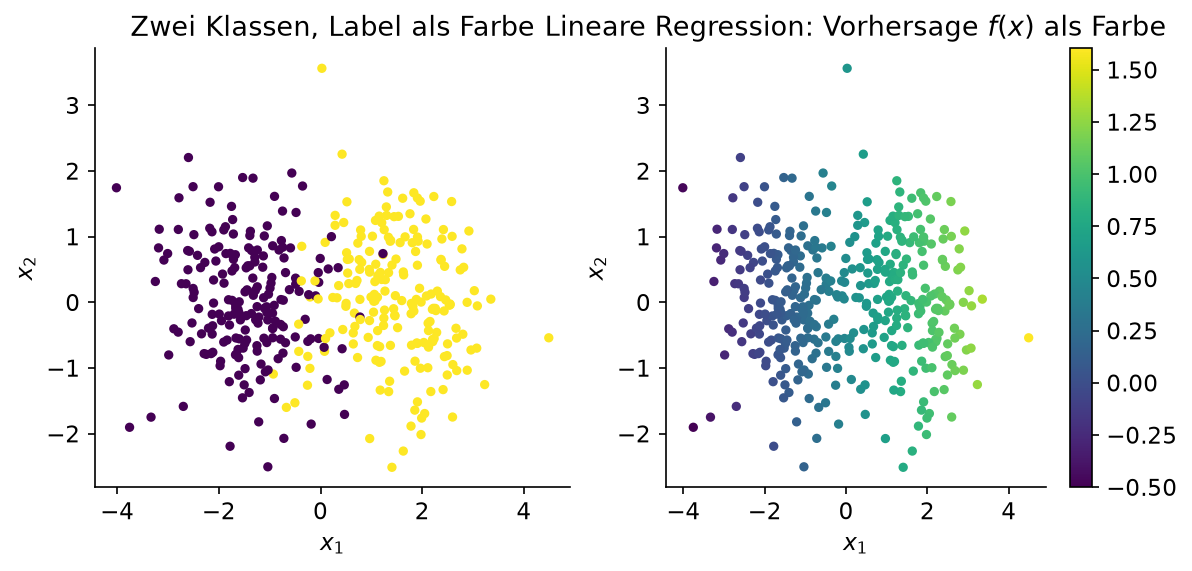
\includegraphics[width=0.64\textwidth]{vl01-blobs-linreg.png}
  \end{center}

  \note{Links zwei linear trennbare Klassen, rechts eine lineare Regression mit der
    Klasse als abhängiger Variable: die Vorhersage ist eine reelle Zahl, die man bei
    $\tfrac12$ abschneiden kann.
    Frage in den Raum: Das funktioniert doch -- was ist daran unbefriedigend?
    Die Antwort (Wahrscheinlichkeitsinterpretation, Ausreißer verschieben die Gerade)
    kommt in VL 4 mit der logistischen Regression. Hier nur die Unzufriedenheit säen.}
\end{frame}

% ------------------------------------------------------------------ Modellgüte
\begin{frame}
  \frametitle{Wie gut ist das Modell?}

  \begin{center}
    \Large Training-Test-Split
  \end{center}

  \bigskip
  \begin{center}
    Accuracy \quad Precision \quad Recall \quad MSE
  \end{center}

  \note{Testset zurückhalten, nur zum Testen benutzen; aufwändiger: $k$-fold
    cross validation. Die vier Maße stehen hier nur als Ankündigung; die Definitionen
    kommen auf der nächsten Folie, und danach zwei Fragen in den Raum.}
\end{frame}

\begin{frame}
  \frametitle{Die vier Maße\pruefungsfrage}

  \begin{columns}[t]
    \begin{column}{0.54\textwidth}
      \textbf{Klassifikation}\\[4pt]
      {\footnotesize Vier Fälle, je nach Wahrheit und Vorhersage:}\\[4pt]
      {\footnotesize
      \begin{tabular}{l|cc}
        & \textbf{sagt positiv} & \textbf{sagt negativ}\\\hline
        \textbf{ist positiv} & TP & FN\\
        \textbf{ist negativ} & FP & TN\\
      \end{tabular}}\\[10pt]
      {\small
      $\text{Accuracy} = \dfrac{\mathrm{TP} + \mathrm{TN}}{\mathrm{TP} + \mathrm{TN} + \mathrm{FP} + \mathrm{FN}}$\\[8pt]
      $\text{Precision} = \dfrac{\mathrm{TP}}{\mathrm{TP} + \mathrm{FP}}$ \quad {\footnotesize\emph{von den gemeldeten}}\\[8pt]
      $\text{Recall} = \dfrac{\mathrm{TP}}{\mathrm{TP} + \mathrm{FN}}$ \quad {\footnotesize\emph{von den vorhandenen}}}
    \end{column}
    \begin{column}{0.44\textwidth}
      \textbf{Regression}\\[4pt]
      {\footnotesize Kein richtig oder falsch, sondern ein Abstand:}\\[10pt]
      {\small $\text{MSE} = \dfrac{1}{N}\displaystyle\sum_{i=1}^{N}\left(y_i - \hat{y}_i\right)^2$}\\[10pt]
      {\footnotesize Quadriert: große Fehler zählen überproportional, das Vorzeichen fällt weg.
      Die Einheit ist die \emph{quadrierte} Zielgröße -- deshalb zieht man oft die Wurzel (RMSE).}
    \end{column}
  \end{columns}

  \note{Die Merkhilfe für die beiden Brüche, die in der Klausur zählt: \textbf{Precision
    hat die Vorhersage im Nenner} (alles, was das Modell gemeldet hat), \textbf{Recall hat
    die Wahrheit im Nenner} (alles, was es hätte finden sollen). Der Zähler ist beide Male
    derselbe, $TP$. Wer das weiß, braucht die Formeln nicht auswendig.
    $TN$ taucht nur in der Accuracy auf -- genau deshalb ist sie bei unbalancierten Klassen
    irreführend: die vielen leichten Negativen dominieren den Bruch.}
\end{frame}

\begin{frame}
  \frametitle{Prüfungsfrage: 99\,\% und trotzdem wertlos}

  \begin{mitmachfrage}
    Ein Spamfilter sieht 1000 Mails, davon sind 10 Spam. Er sagt bei \emph{jeder}
    Mail „kein Spam“.\\[6pt]
    Welche Werte hat es?
    \optionen{Accuracy 99\,\%, Recall 0\,\%}{Accuracy 0\,\%, Recall 99\,\%}%
             {beide 99\,\%}{beide 0\,\%}
  \end{mitmachfrage}
  \pause
  \vfill
  \antwort A. 990 von 1000 richtig, das sind 99\,\% Accuracy -- ohne dass das Modell
  irgendetwas gelernt hat. Gefunden hat es von den 10 Spam-Mails keine einzige:
  $\mathrm{TP} = 0$, also Recall $= 0/10 = 0\,\%$. Die Precision ist hier nicht einmal definiert
  ($0/0$): Das Modell meldet nichts, worüber man urteilen könnte.

  \note{Das ist der Klassiker, und er lohnt die zwei Minuten. Pointe: \emph{Eine einzelne
    Zahl kann ein Modell nicht beschreiben.} Accuracy allein sagt bei unbalancierten Klassen
    nichts; deshalb nennt man Precision und Recall immer als Paar.
    Wenn jemand fragt, warum Precision undefiniert ist und nicht null: Der Nenner $\mathrm{TP}+\mathrm{FP}$
    ist null, es gibt keine Meldung. In sklearn kommt per Konvention 0 heraus, mit Warnung.}
\end{frame}

\begin{frame}
  \frametitle{Prüfungsfrage: nachrechnen\pruefungsfrage}

  \begin{mitmachfrage}
    Ein Rissdetektor prüft 200 Bauteile. Er meldet 30 als „rissig“, davon sind 24
    tatsächlich rissig. Insgesamt gibt es 40 rissige Bauteile.\\[6pt]
    Precision und Recall?
    \optionen{$0{,}80$ und $0{,}60$}{$0{,}60$ und $0{,}80$}%
             {$0{,}80$ und $0{,}12$}{$0{,}12$ und $0{,}60$}
  \end{mitmachfrage}
  \pause
  \vfill
  \antwort A. $\mathrm{TP} = 24$, gemeldet $= 30$, vorhanden $= 40$.
  Precision $= 24/30 = 0{,}80$, Recall $= 24/40 = 0{,}60$.
  Die 200 braucht man für beides \emph{nicht} -- sie steht nur da, um zu prüfen, ob man
  den richtigen Nenner nimmt.

  \note{Dieselben Zahlen stehen als Übungsaufgabe im Kapitel, dort ohne Lösung mit
    Antwortprobe („die beiden Werte verhalten sich wie 4 zu 3“).
    Die Nachfrage, die sich lohnt: \emph{Welche der beiden Zahlen gewichten Sie in der
    Qualitätssicherung höher?} Recall -- ein übersehener Riss geht ins Produkt, ein
    Fehlalarm kostet nur eine zweite Prüfung. In der Spam-Erkennung ist es umgekehrt:
    Dort tut ein Fehlalarm weh, weil eine echte Mail im Spam-Ordner landet.
    Das ist der Übergang zur nächsten Folie: Es gibt keine Güte an sich, nur Güte für
    einen Zweck.}
\end{frame}

\begin{frame}
  \frametitle{Quizfrage}

  \begin{center}
    \Large Was passiert mit dem Testset,\\[6pt]
    wenn ich damit Modelle vergleiche\\[6pt]
    und Hyperparameter optimiere?
  \end{center}

  \note{\textbf{Nicht auflösen, sammeln.} Das ist der dialogischste Moment der Sitzung,
    2025 gut zehn Minuten wert.
    Erwartbare Antworten: Sampling-Bias; Overfitting auf das Testset. Den scheinbaren
    Widerspruch ausdrücklich stehen lassen, bis jemand den \emph{indirekten} Fit
    erklärt: ich wähle die Hyperparameter nach dem Testergebnis, also fließt das
    Testset doch ins Modell ein.
    Erst dann die Pointe: Validation-Split -- und das Stichwort Spillover.}
\end{frame}

\begin{frame}
  \frametitle{Training, Validation, Test}

  \begin{center}
    \Large
    Training \qquad Validation \qquad Test\\[14pt]
    \normalsize
    Modelle vergleichen, Hyperparameter wählen: am \emph{Validation}-Set.\\[6pt]
    Das Testset \emph{einmal} anfassen -- ganz am Ende.
  \end{center}

  \note{Erst umblättern, wenn die Pointe im Hörsaal gefallen ist. Wer die Hyperparameter
    nach dem Testergebnis wählt, lässt das Testset indirekt ins Modell einfließen
    (Spillover), und die gemessene Güte ist zu optimistisch. Deshalb vom Trainingsset ein
    drittes Stück abspalten, daran vergleichen und wählen; das Testset bleibt für die eine
    Zahl am Ende. Steht im Skript direkt hinter der Quizfrage, und im Glossar.}
\end{frame}

% ------------------------------------------------------------------ Lesetext
% Umgebaut am 2026-10-14. Vorher: drei Peer-Instruction-Fragen zu einem Artikel, den
% im Hörsaal noch niemand gelesen hatte -- ein Quiz über unbekannten Stoff, und die
% „Fragen" waren Themen („GPU oder SIMD?"), keine Fragen. Jetzt drei Takte:
% zitierter Absatz (der Gegenstand), eine daraus beantwortbare Frage, Leseauftrag.
\begin{frame}
  \frametitle{Lesetext: AMD und der CUDA-Graben}

  {\small Doug Eadline, \emph{How AMD May Get Across the CUDA Moat}, HPCwire,
  5.\,Oktober 2023 -- der erste Absatz:}

  \medskip
  \begin{beamerboxesrounded}[upper=mitmachtitel,lower=mitmachkoerper,shadow=false]{Zitat}
    \small
    When discussing GenAI, the term ``GPU'' almost always enters the conversation and the
    topic often moves toward performance and access. Interestingly, the word ``GPU'' is
    assumed to mean ``Nvidia'' products. (As an aside, the popular Nvidia hardware used in
    GenAI are not technically Graphical Processing Units. I prefer SIMD units.)
  \end{beamerboxesrounded}

  \medskip
  {\footnotesize\url{https://www.hpcwire.com/2023/10/05/how-amd-may-get-across-the-cuda-moat/}}

  \note{\textbf{Eine Minute: vorlesen oder lesen lassen, nicht kommentieren.} Der Absatz
    ist der Gegenstand der nächsten Folie, nicht Dekoration.
    Worauf man zeigen kann, wenn jemand stockt: Der Autor behauptet zweierlei. Erstens,
    dass „GPU“ im GenAI-Gespräch stillschweigend „Nvidia“ heißt. Zweitens -- im Nebensatz,
    fast beiläufig -- dass die Dinger gar keine Grafikprozessoren seien.
    Genau dieser Nebensatz ist die Aufgabe auf der nächsten Folie.
    Zitiert mit Quelle und Link (Zitatrecht, §51 UrhG: der Absatz ist Gegenstand der
    Erörterung, nicht Schmuck). Der Rest des Artikels bleibt Hausaufgabe.}
\end{frame}

\begin{frame}
  \frametitle{``I prefer SIMD units'' -- warum?\pruefungsfrage}

  \begin{mitmachfrage}
    Warum ist die Nvidia-Hardware im Rechenzentrum \emph{technisch} keine
    \emph{Graphics} Processing Unit?
    \optionen{Marketing: „GPU“ klingt nur besser}%
             {SIMD ist das Prinzip, GPU das Produkt -- diese Chips geben nie ein Bild aus}%
             {SIMD ist Nvidias interner Produktname}%
             {Die Karten können gar keine Grafik}
  \end{mitmachfrage}
  \pause
  \vfill
  {\small
  \antwort B. \textbf{SIMD} (\emph{single instruction, multiple data}) ist ein
  \emph{Rechenprinzip}: dieselbe Operation gleichzeitig auf vielen Datenelementen. Die
  \textbf{GPU} ist ein \emph{Produkt}, das es mit tausenden kleinen Kernen umsetzt --
  ursprünglich, um Bildpunkte parallel zu berechnen.\\[4pt]
  Fürs Deep Learning zählt nur das Prinzip, denn Matrixmultiplikation \emph{ist}
  SIMD-Arbeit. Deshalb trainiert auch eine Gaming-Karte -- und deshalb sind die Chips im
  Rechenzentrum, die nie ein Bild ausgeben, keine \emph{Graphics} Processing Units mehr.}

  \note{\textbf{Drei bis vier Minuten.} Das ist die einzige Frage des Blocks, die der
    Hörsaal \emph{beantworten kann} -- die Antwort steht im Absatz der vorigen Folie, man
    muss sie nur ausbuchstabieren. Genau deshalb steht sie hier und die anderen beiden
    Fragen nicht: Die bräuchten den ganzen Artikel.
    D ist der lehrreiche Falschanker: Die Karten \emph{können} Grafik, sie tun es im
    Rechenzentrum nur nie. 2025 kam aus dem Hörsaal eine gute Antwort über Raster und
    Shader gegen Rechenzentrum -- die lohnt sich abzuwarten, bevor man weiterklickt.
    Merksatz, der bleiben soll: \emph{SIMD ist das Prinzip, die GPU das Produkt.}}
\end{frame}

\begin{frame}
  \frametitle{Leseauftrag bis nächste Woche}

  \begin{center}
    {\small Doug Eadline, \emph{How AMD May Get Across the CUDA Moat} (HPCwire, 2023)}\\[4pt]
    {\footnotesize\url{https://www.hpcwire.com/2023/10/05/how-amd-may-get-across-the-cuda-moat/}}
  \end{center}

  \bigskip
  Zwei Fragen, die der Artikel beantwortet:
  \medskip
  \begin{enumerate}\setlength{\itemsep}{6pt}
  \item Wer entwickelt \textbf{PyTorch} -- und warum steht das in einem Artikel über AMD?
  \item Was ist der \emph{moat}, der Burggraben, aus dem Titel: \textbf{CUDA} oder \textbf{ROCm}?
  \end{enumerate}

  \bigskip
  {\small Antworten zum Selbstkontrollieren: im Skript, Kapitel 1, Box
  \emph{„Antworten zum Lesetext“}.}

  \note{\textbf{Eine Minute, am Stück ansagen.} Das ist der Leseauftrag, nicht noch eine
    Quizrunde -- die beiden Fragen setzen den ganzen Artikel voraus.
    Kurz dazusagen, worauf die Antworten hinauslaufen, damit das Lesen eine Richtung hat:
    PyTorch gehört \emph{nicht} Nvidia (Facebook AI Research, heute Meta, seit 2022 unter
    der Linux Foundation) -- deshalb kann es überhaupt ein anderes Backend ansprechen, und
    genau das ist AMDs Hebel. Und der Graben ist \emph{nicht die Hardware, sondern die
    Software drumherum}: CUDA ist seit 2007 der De-facto-Standard, ROCm kam später und hat
    weniger fertige Bibliotheken.
    Wer mehr will: Die Antwortbox im Skript ist ausführlicher als alles, was hier in drei
    Minuten ginge.}
\end{frame}

% ------------------------------------------------------------------ Geschichte
\begin{frame}
  \frametitle{Kurzgeschichte: bis 2010}

  \begin{columns}[c]
    \begin{column}{0.52\textwidth}
      \begin{itemize}\setlength{\itemsep}{8pt}
      \item[\textbf{1943}] McCulloch \& Pitts
      \item[\textbf{1958}] Rosenblatt: Perzeptron
      \item[\textbf{1969}] Minsky \& Papert $\Rightarrow$ AI Winter
      \item[\textbf{1986}] Backpropagation
      \end{itemize}
    \end{column}
    \begin{column}{0.46\textwidth}
      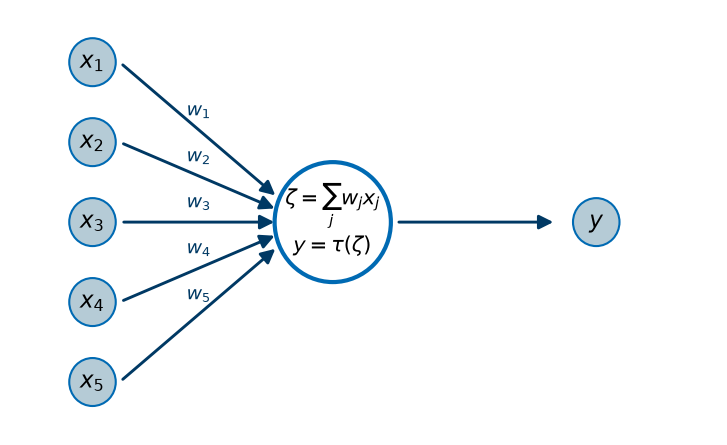
\includegraphics[width=\textwidth]{vl01-neuron.png}
    \end{column}
  \end{columns}

  \note{1943: ein Hirnneuron, modelliert mit elektrischen Schaltkreisen.
    1958: das Perzeptron wurde tatsächlich \emph{gebaut} -- Bild auf der nächsten Folie.
    1969: nur linear trennbare Klassen -- gilt als Auslöser des ersten AI Winter.
    1986: Backpropagation macht mehr Schichten praktikabel -- unser VL 6.}
\end{frame}

\begin{frame}
  \frametitle{1958: gebaut, nicht simuliert}

  \begin{columns}[c]
    \begin{column}{0.48\textwidth}
      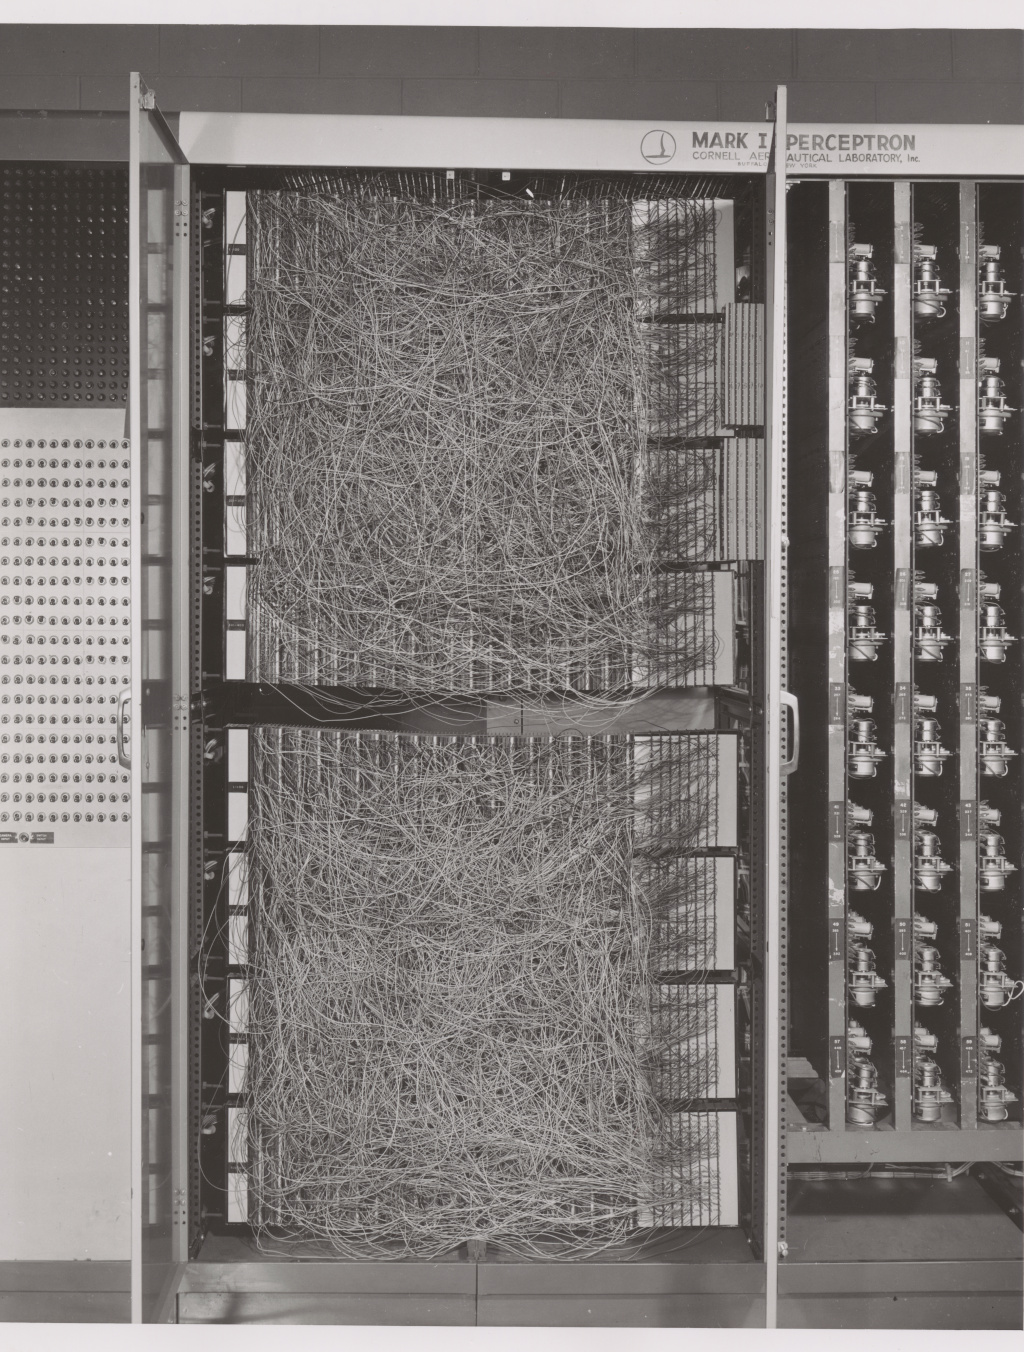
\includegraphics[height=0.58\textheight]{vl01-mark-i-perceptron.jpg}
    \end{column}
    \begin{column}{0.48\textwidth}
      Der Mark I Perceptron am Cornell Aeronautical Laboratory in Buffalo.\\[14pt]
      Fotozellen als Eingabe,\\
      Potentiometer als Gewichte,\\
      Elektromotoren zum Nachstellen.\\[14pt]
      {\footnotesize Foto: Cornell Aeronautical Laboratory / Cornell University Library.}
    \end{column}
  \end{columns}

  \note{Das ist der Aufhänger für nächste Woche: die Gewichte waren Drehwiderstände,
    das Training war ein Motor, der sie verstellt. Wer das Bild einmal gesehen hat,
    versteht „Gewicht“ nicht mehr als abstrakte Zahl.
    Im Bild: in der Mitte das Steckbrett, das die Fotozellen mit den
    Assoziationseinheiten verdrahtet, rechts die Reihen von Potentiometern, also die
    Gewichte. Bildnachweis in \texttt{slides/README.md}.
    Wer mehr will: Olazaran, M. (1996), \emph{A Sociological Study of the Official History
    of the Perceptrons Controversy} -- zeigt, dass die Erzählung vom AI Winter durch
    Minsky und Papert so glatt nicht stimmt. Steht im Skript.}
\end{frame}

\begin{frame}
  \frametitle{Kurzgeschichte: 2010--2015}

  \begin{columns}[c]
    \begin{column}{0.56\textwidth}
      \begin{itemize}\setlength{\itemsep}{10pt}
      \item[\textbf{2012}] AlexNet: ein CNN gewinnt ImageNet \hfill {\small VL 11}
      \item[\textbf{2013}] word2vec: Wörter als Vektoren \hfill {\small VL 9}
      \item[\textbf{2014}] GANs: zwei Netze im Wettstreit \hfill {\small VL 13}
      \end{itemize}
    \end{column}
    \begin{column}{0.42\textwidth}
      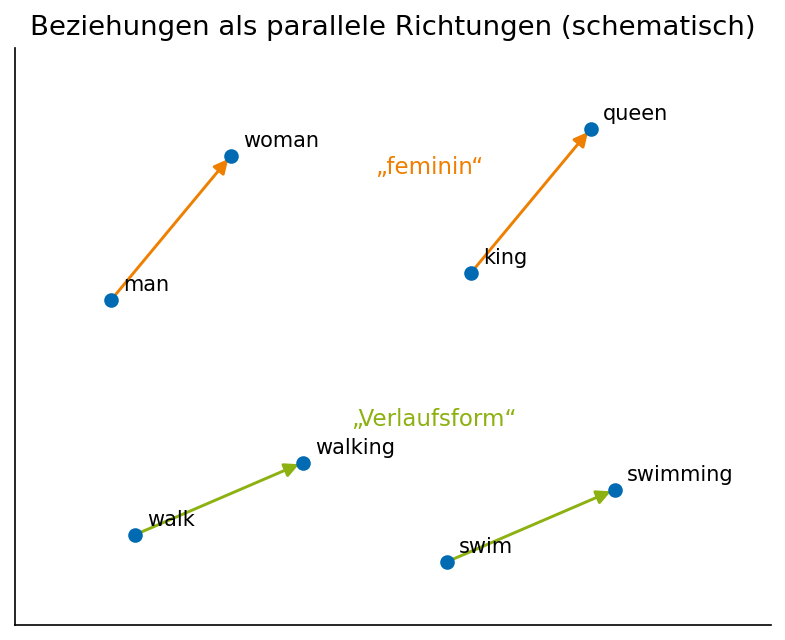
\includegraphics[width=\textwidth]{vl13-word-arithmetic.png}
    \end{column}
  \end{columns}

  \note{AlexNet: „the paper that sparked the field of Deep Learning“ -- ein CNN
    gewinnt ImageNet mit großem Abstand, trainiert auf GPUs.
    word2vec: Wörter als Vektoren in einem latenten Raum; das Bild ist die
    Wortarithmetik aus VL 9 (king $-$ man $+$ woman $\approx$ queen), hier nur als
    Appetithappen. Bis zum 2026-10-02 standen hier drei Briefmarken, von denen keine
    lesbar war.
    GANs: zwei Netze im Wettstreit, erstmals „realistische“ Bildgenerierung.
    Alle drei kommen wieder, deshalb die VL-Nummern daneben.
    Lesetipp: „The Decade of Deep Learning“ von Leo Gao.}
\end{frame}

\begin{frame}
  \frametitle{Kurzgeschichte: nach 2015}

  \begin{itemize}\setlength{\itemsep}{8pt}
  \item[\textbf{2017}] Transformer \hfill {\small VL 10, aber wir trainieren keine}
  \item[\textbf{2020}] AlphaFold 2
  \item[\textbf{2021}] Diffusionsmodelle schlagen GANs
  \item[\textbf{2022}] ChatGPT
  \item[\textbf{2024/25}] Agentic Coding \hfill {\small VL 15}\\[3pt]
    {\footnotesize Claude 3.5 Sonnet, GPT-4.1, Gemini 2.5 Pro, Qwen3-Coder, Kimi K2:\\
    je $\gtrsim 50\,\%$ auf SWE-bench Verified}
  \end{itemize}

  \note{Transformer: „Attention is all you need“, Grundlage für GPT -- wir schauen
    sie in VL 10 an, trainieren aber keine.
    AlphaFold 2 „löst“ das Proteinfaltungsproblem, Nobelpreis Chemie 2024.
    Diffusion: das Verfahren (DDPM) ist von 2020; 2021 schlägt es die GANs bei der
    Bildqualität (Dhariwal und Nichol, „Diffusion Models Beat GANs on Image Synthesis“).
    Nach ChatGPT: RLHF, Copilot, Multimodalität, RAG, Agents.
    \textbf{Agentic Coding}: SWE-bench Verified ist die von OpenAI 2024 geprüfte
    500-Aufgaben-Teilmenge von SWE-bench -- echte GitHub-Issues aus Python-Projekten,
    bestanden ist eine Aufgabe erst, wenn die Tests des Projekts durchlaufen. Der Sprung
    ist der eigentliche Punkt: 2023 lagen die besten Systeme im niedrigen einstelligen
    Bereich, binnen zwei Jahren liegt ein halbes Dutzend Modelle darüber -- offene
    (Qwen3-Coder, Kimi K2) wie geschlossene. \emph{Die Prozentzahlen vor der Sitzung
    nachsehen, sie altern schneller als jede andere Zahl im Deck}; die Rangfolge wechselt
    monatlich, die Größenordnung nicht. Anschluss an VL 15 (Vibecoding).
    Ehrlich bleiben: das meiste davon ist Stoff der aufbauenden Module im Master.}
\end{frame}

% ------------------------------------------------------------------ Abschluss
\begin{frame}
  \frametitle{Take-Home}

  \begin{center}
    \Large
    Deep Learning = Machine Learning mit \emph{tiefen} Netzen.\\[14pt]
    \pause % Transition 2026-10-14: die drei Sätze einzeln landen lassen
    Ein generatives Modell ist ein Modell einer \emph{Verteilung}.\\[14pt]
    \pause
    Supervised: eine Spalte, die ich später \emph{nicht mehr bekomme}.
  \end{center}

  \note{Zwei Minuten, die drei Take-Home-Sätze der Sitzung 2025. Der erste nimmt dem
    Begriff die Magie, der zweite ist der Haken für Autoencoder, VAE und GANs, der dritte
    für alles, was Regression oder Klassifikation heißt.}
\end{frame}


% ------------------------------------------------------------------ Themenfelder
\begin{frame}
  \frametitle{Drei Fragen für dieses Semester}

  \begin{itemize}\setlength{\itemsep}{14pt}
  \item[\textbf{A}] Wie \emph{arbeitet} ein Neuron, wie ein neuronales Netz?
  \item[\textbf{B}] Wie \emph{trainiert} man ein neuronales Netz?
  \item[\textbf{C}] Wie \emph{setzt} man neuronale Netze \emph{ein}?
  \end{itemize}

  \bigskip
  \begin{center}
    Wir behandeln die drei verschränkt -- angefangen mit \textbf{A}.
  \end{center}

  \note{Die Folie ist der Kompass für das Semester: Wer sich später fragt, wozu eine
    Sitzung gut ist, sortiert sie hier ein.
    Grobe Zuordnung, falls jemand nachfragt -- \textbf{A} ist VL 2--4 (Neuron, Perzeptron,
    vortrainierte Modelle, Tensoren), \textbf{B} ist der lange Mittelteil VL 4--9
    (logistische Regression, Loss, Gradientenabstieg, Backpropagation, Autograd, Netze von
    Hand), \textbf{C} ist VL 10--15 (CNN, Transformer, LLMs benutzen, GANs, latente Räume,
    Destillation).
    \textbf{Warum verschränkt und nicht der Reihe nach}: Ohne ein trainiertes Netz kann man
    nichts einsetzen, aber ohne etwas Eingesetztes bleibt das Training abstrakt. Deshalb
    kommen vortrainierte Modelle schon in VL 3 -- da ist von B noch nichts behandelt, und
    trotzdem tut das Netz etwas Sichtbares. Das ist Absicht, keine Unordnung.}
\end{frame}

\begin{frame}
  \frametitle{In die Praxis}

  \begin{itemize}\setlength{\itemsep}{8pt}
  \item Morgen 10:30: Übung -- ein Blatt zum Warmwerden, gemeinsam, ohne Abgabe
  \item Ab heute: erstes Abgabeblatt -- lineare Algebra, NumPy; Abgabe nächsten Mittwoch
  \item Danach: Perzeptron in NumPy
  \end{itemize}

  \bigskip
  \begin{center}
    Nächste Woche: \emph{Neuron und Perzeptron}.
  \end{center}

  \note{Zwei Minuten. Ausdrücklich ansagen, was auf dem ersten Abgabeblatt steht (lineare
    Algebra, dazu kleine NumPy- und Matplotlib-Aufgaben) und dass das Perzeptron erst auf dem
    nächsten Blatt programmiert wird -- das hat 2025 Rückfragen erspart.
    Und: Die Eingangsumfrage schließt in ILIAS um 13:55, also mit dieser Sitzung -- wer
    sie noch nicht ausgefüllt hat, tut es jetzt, nicht morgen.}
\end{frame}

% ------------------------------------------------------------------ Schluss
\begin{frame}
  \frametitle{Danke für Ihre Aufmerksamkeit}
  \framesubtitle{Fragen?}

  \textbf{Weiterlesen} -- beides frei verfügbar und im Skript pro Kapitel verlinkt:
  \begin{itemize}\setlength{\itemsep}{4pt}
  \item Prince, \emph{Understanding Deep Learning}
  \item Deisenroth, Faisal, Ong, \emph{Mathematics for Machine Learning}
  \end{itemize}

  \bigskip
  \begin{itemize}\setlength{\itemsep}{4pt}
  \item Skript: {\small\url{voelkel.pages.cs.uni-duesseldorf.de/eidl-skript/}}
  \item Fragen außerhalb der Vorlesung: Rocket.Chat \texttt{\#eidl-2026}
  \end{itemize}

  \note{Die Schlussfolie bleibt stehen, solange Fragen kommen -- deshalb steht alles
    darauf, was jemand nach der Sitzung braucht.
    Die Umfrage steht bewusst \emph{nicht} mehr hier: Sie schließt mit dieser Sitzung
    (ILIAS-Run-Datei \texttt{ilias/runs/ws2026-27.yaml}, \texttt{survey-entry}:
    bis 14.10.2026 13:55), die Ansage dazu gehört auf die Folien
    \emph{Eingangsumfrage} und \emph{In die Praxis}, nicht auf eine Folie, die ein
    Semester lang im Netz steht.}
\end{frame}

\end{document}

%%% Local Variables:
%%% mode: latex
%%% TeX-master: t
%%% End:
